
\paragraph{Pipeline}\label{par:pipeline}

En el proceso de Pull Request tal y como se diseño\ref{par:testing} se ejecuta el pipeline diseñado para garantizar la entrega de software testeado y con el estandar de calidad requerido. Podemos ver en la figura\ref{fig:githubActions} que los pasos son:

\begin{itemize}
    \item ejecutar los tests
    \item pasar el chequeo de estandar del código
    \item compilar en modo producción
\end{itemize}

faltarían el CD o continous delivery que ejecutaría los pasos de subir dicho ejecutable a un servidor, al menos para el programa manager.

\begin{figure}[H]
    \centering
    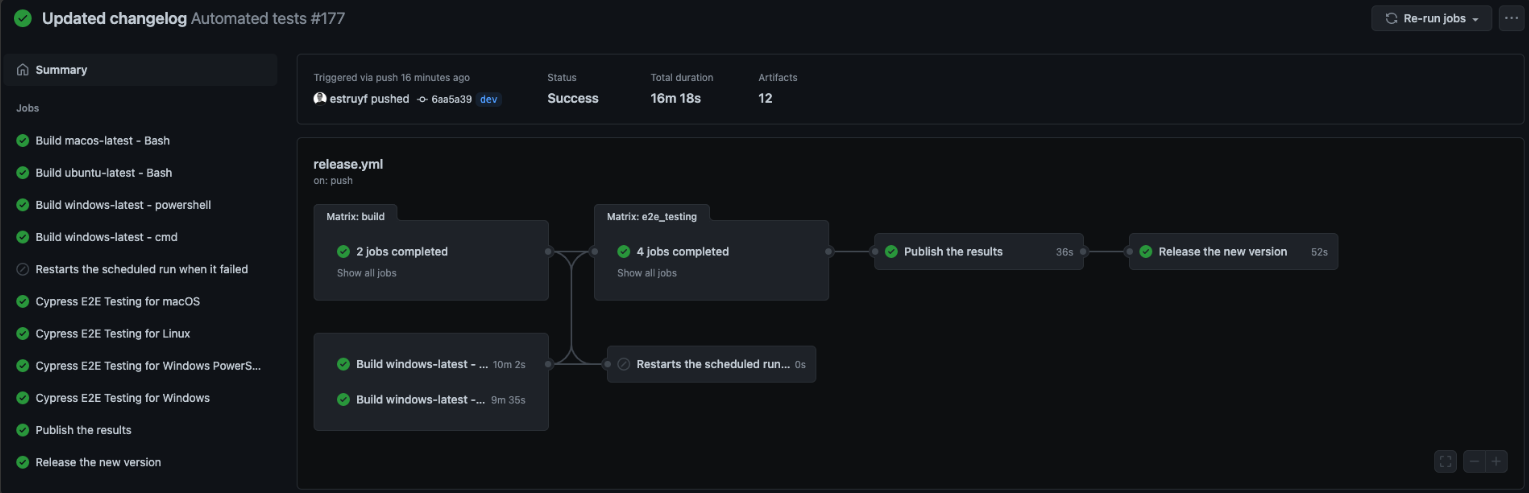
\includegraphics[height=0.2\textheight]{./part/Ejecucion/Seguimiento/PuestaAPunto/img/githubPipelines}
    \caption{pipeline en Github}\label{fig:githubActions}
\end{figure}

\paragraph{Montaje de prueba}\label{par:montaje}

Para la prueba conjunta del sistema se ha desplegado un montaje como se ve en la figura\ref{fig:Control-Diagrama UML de despliegue}

\begin{figure}[H]
    \centering
    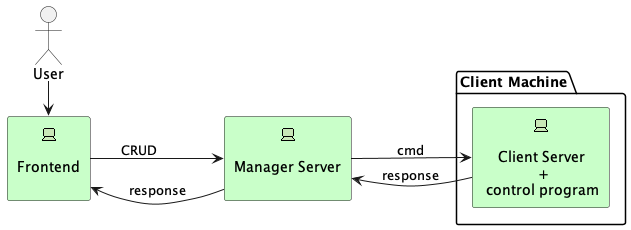
\includegraphics[height=0.2\textheight]{./part/Ejecucion/Seguimiento/PuestaAPunto/img/deploy}
    \caption{diagrama de despliegue de prueba}\label{fig:despliegue de prueba}
\end{figure}

Podemos ver en la imagen\ref{fig:montaje en protoboard} el montaje físico de conexión entre el el servidor cliente, en este caso una Rashpberry con la protoboard donde tenemos la conexión con el puente H y el motor de corriente continua.

\begin{figure}[H]
    \centering
    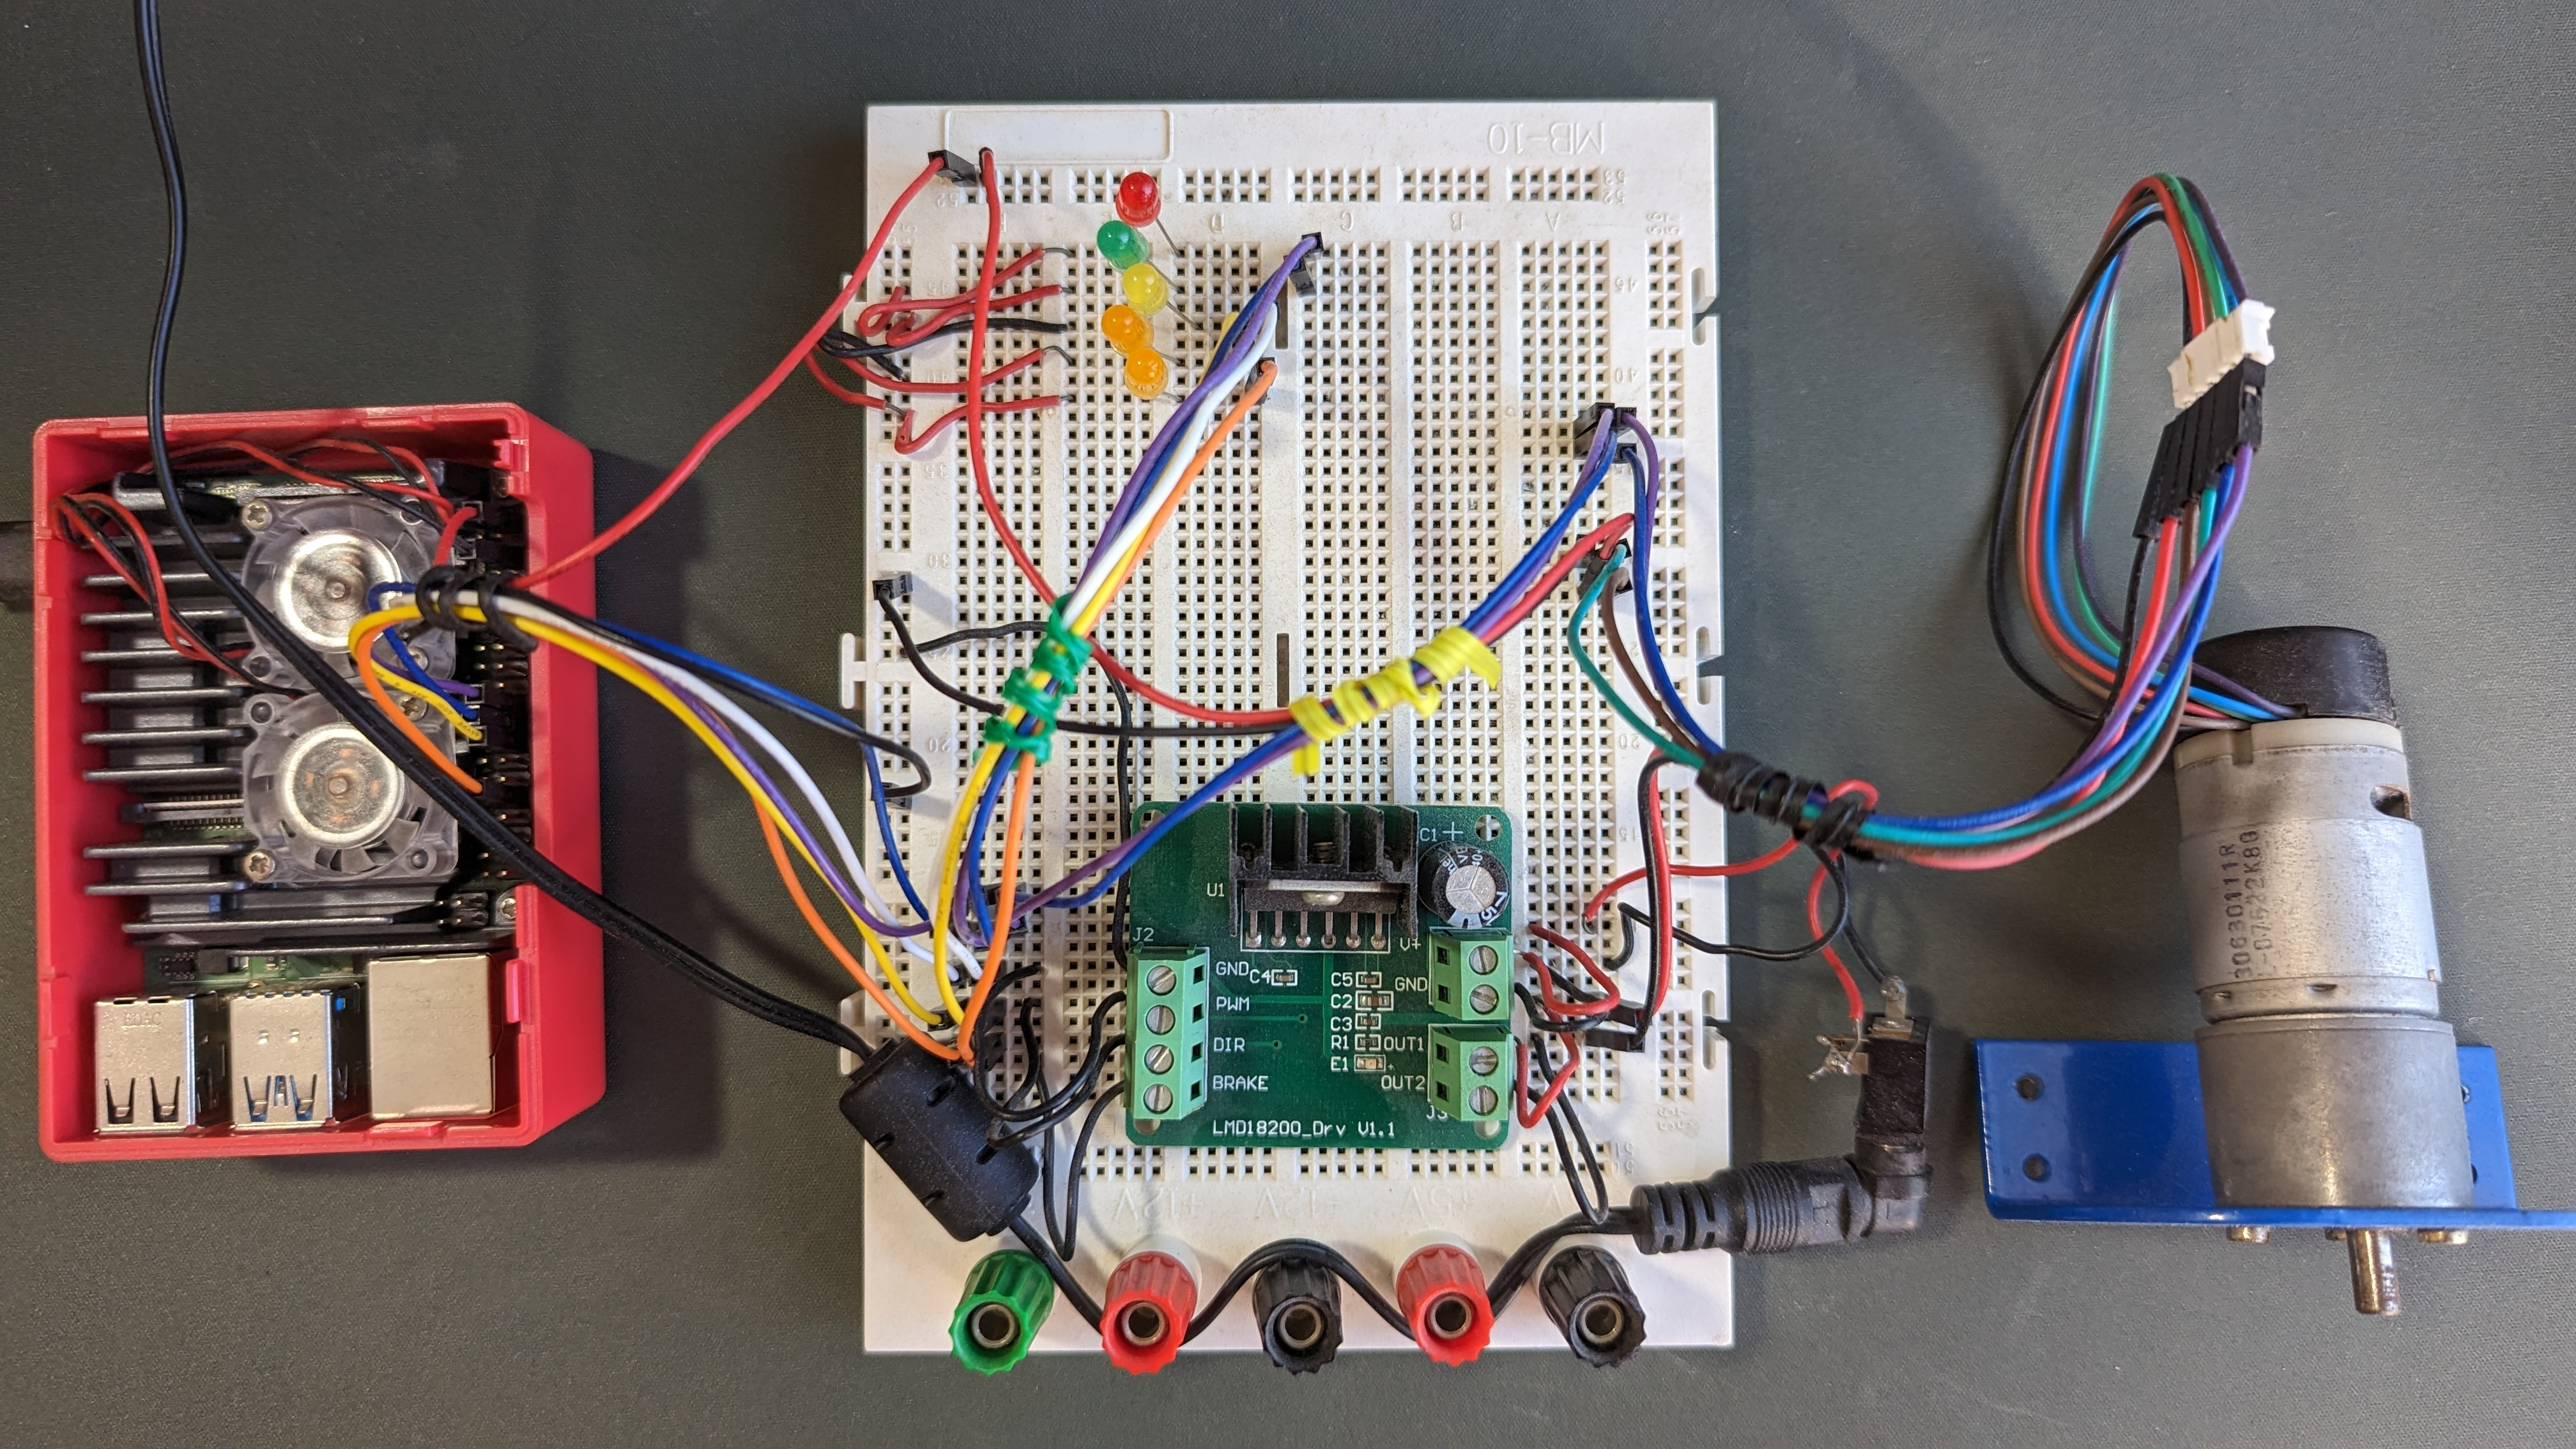
\includegraphics[height=0.2\textheight]{./part/Ejecucion/Seguimiento/PuestaAPunto/img/montajeProtoboard}
    \caption{montaje en protoboard}\label{fig:montaje en protoboard}
\end{figure}

\paragraph{Interfaz gráfica}\label{par:interfaz}

Para controlar el programa manager se ha desarrollado como añadido una interfaz gráfica. En la figura \ref{fig:frontend} podemos ver el listado de las tareas creadas, el estado en el que se encuentran y un boton para ejecutar manualmente las que son manuales.

\begin{figure}[H]
    \centering
    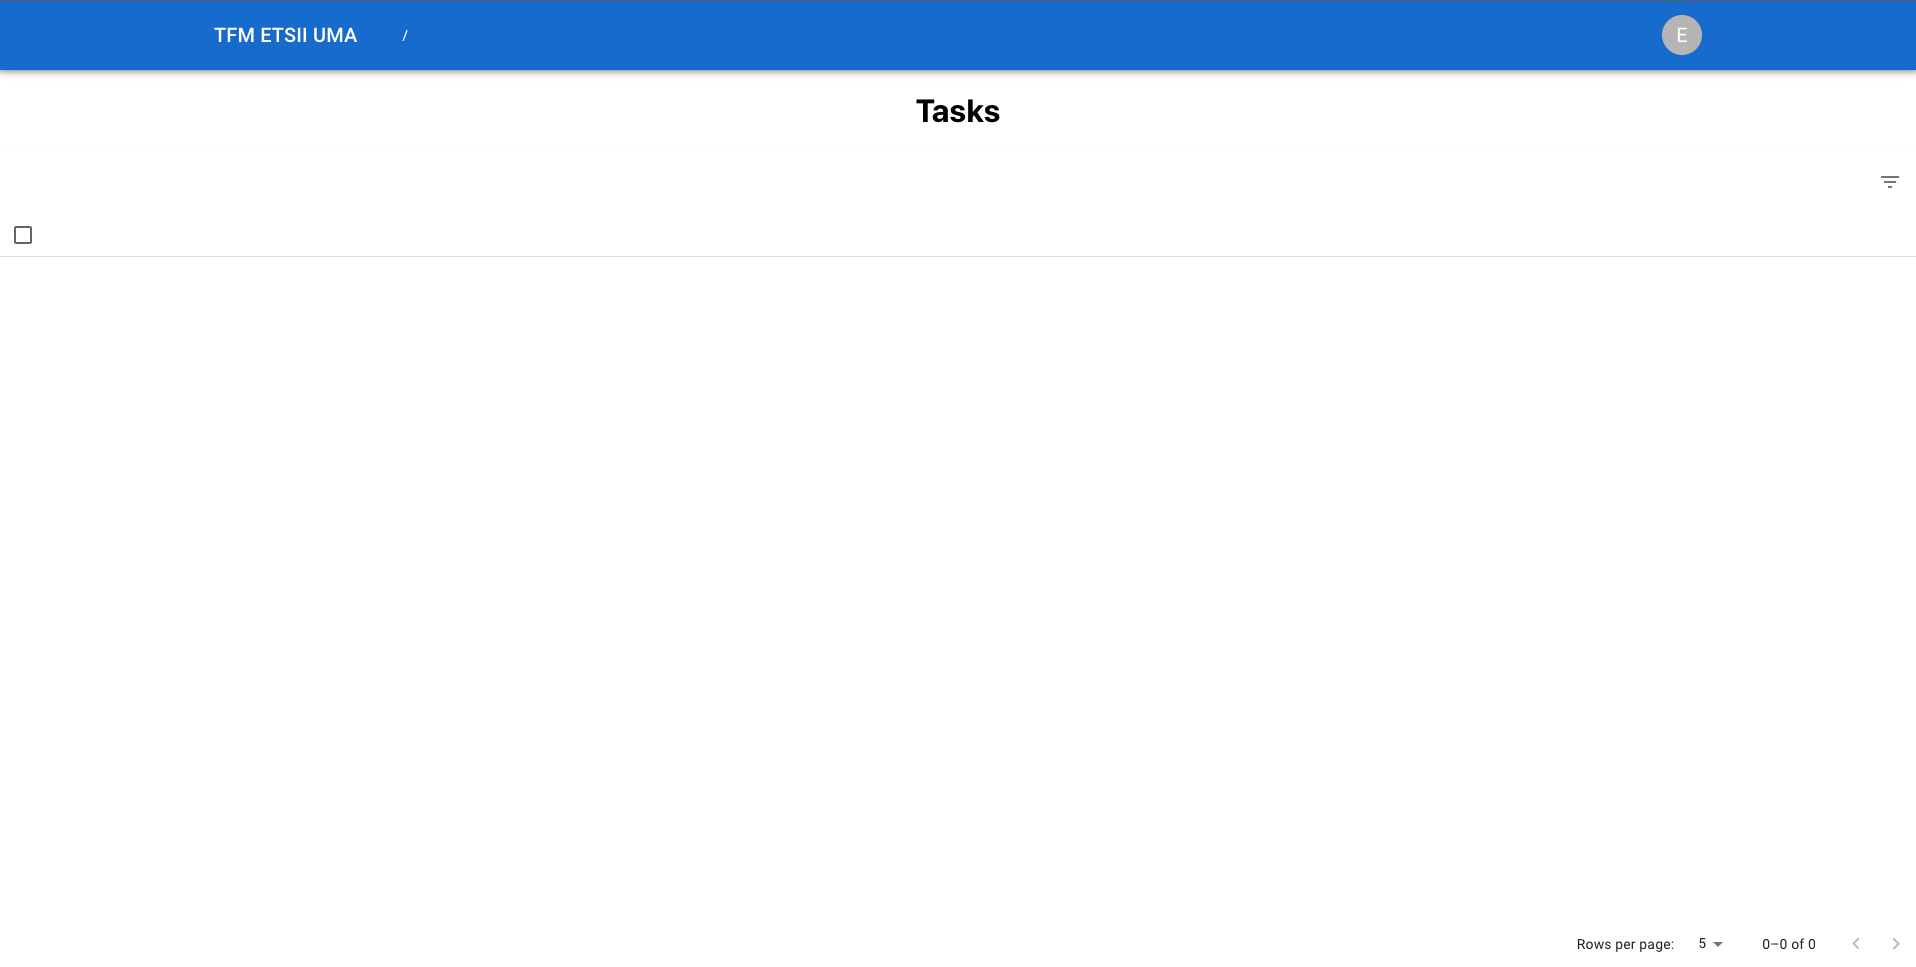
\includegraphics[height=0.2\textheight]{./part/Ejecucion/Seguimiento/PuestaAPunto/img/frontend}
    \caption{frontend: task list}\label{fig:frontend}
\end{figure}

Para ejecutar manualmente una tarea disponimos de una gráfica para ver en tiempo real la evolución de la variable controlada.

\begin{figure}[H]
    \centering
    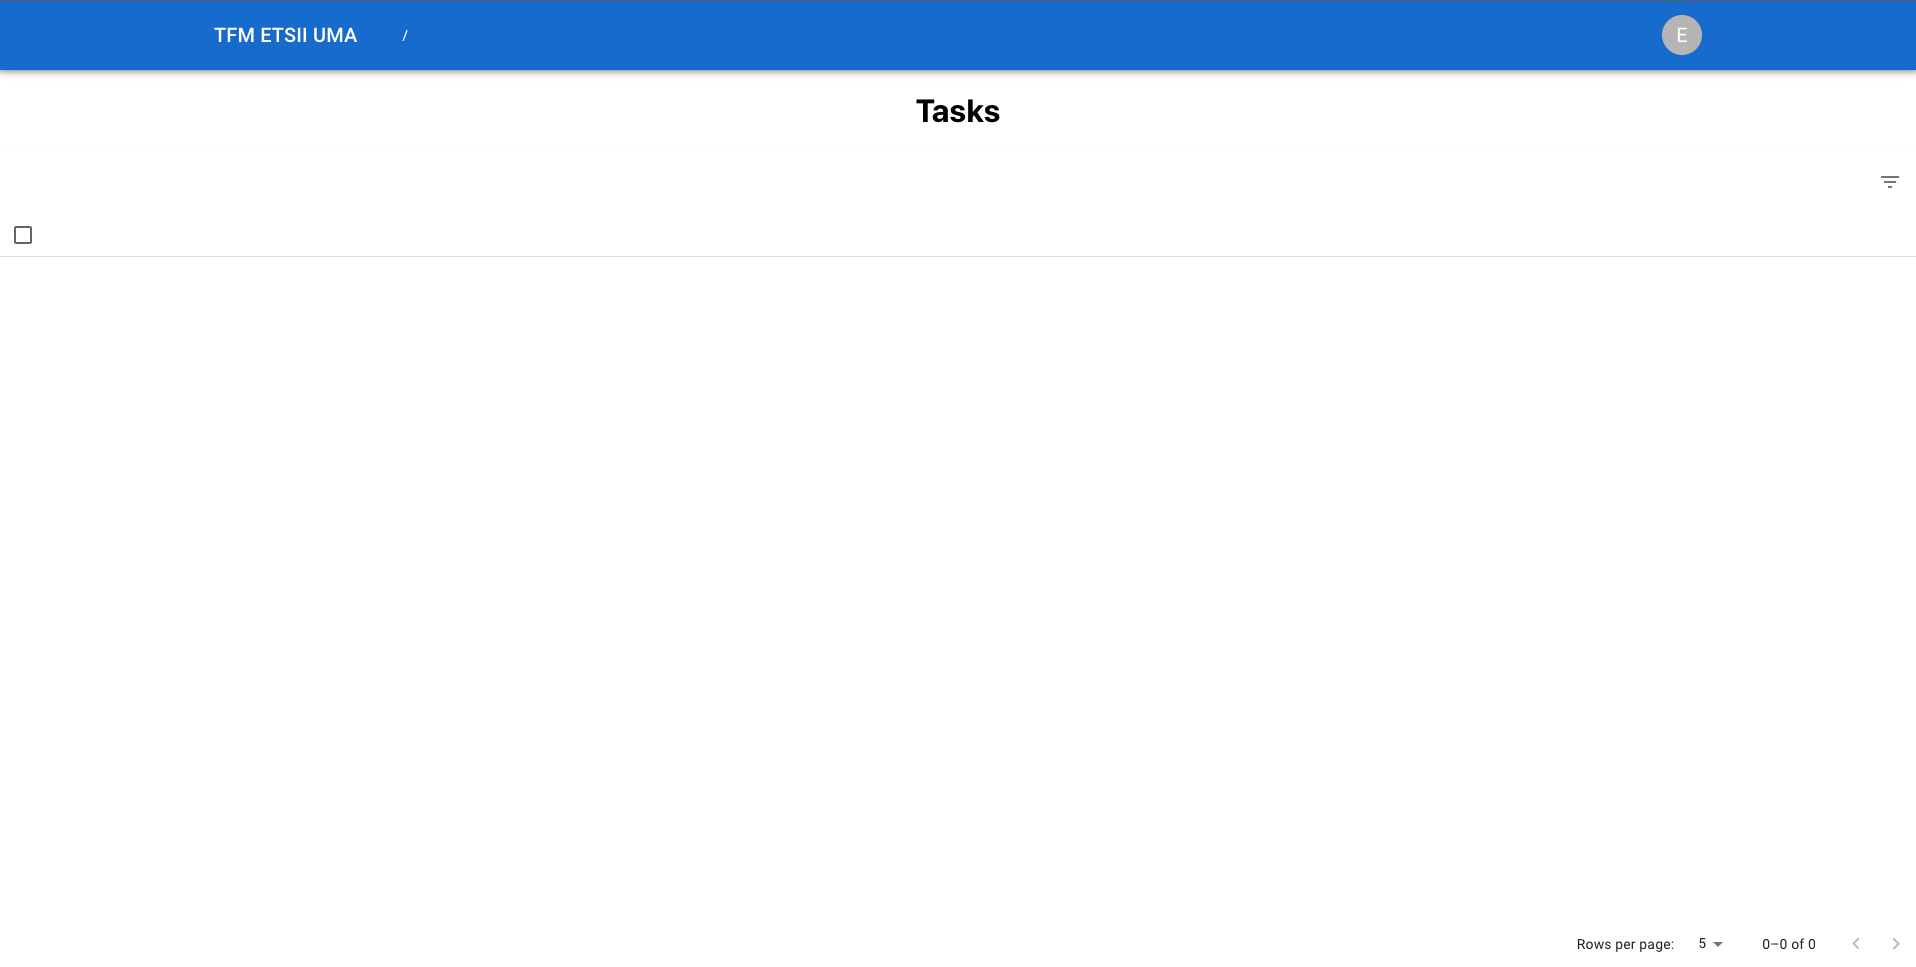
\includegraphics[height=0.2\textheight]{./part/Ejecucion/Seguimiento/PuestaAPunto/img/runner}
    \caption{frontend: runner}\label{fig:runner}
\end{figure}